\documentclass{beamer}
%\usepackage[latin1]{inputenc}
%\usepackage{lmodern}
\usepackage{times}
\usepackage[T1]{fontenc}
\usepackage{graphicx}
\usepackage{bm}
\usepackage{tikz}
\usepackage{verbatim}
\usepackage{amsmath}
\usepackage{booktabs}
\usepackage[small,labelformat=empty]{caption}
\usepackage{url}
\usepackage{colortbl}
%\usetikzlibrary{circuits}
\usetikzlibrary{automata,positioning}


\usetheme{Frankfurt}
%\usetheme{Warsaw}
\title[Title of presentation]{Title of presentation\\
{\small possibly subtitle}
}
\author[author name]
{further information <\url{can-include.urls}>}
\institute[Fnord GmbH]{}
\date{23.5.1984 - 42.5.1984}

\begin{document}

\section{uhrenbaustein}
  \begin{frame}{uhrenbaustein - integrate modules}
	  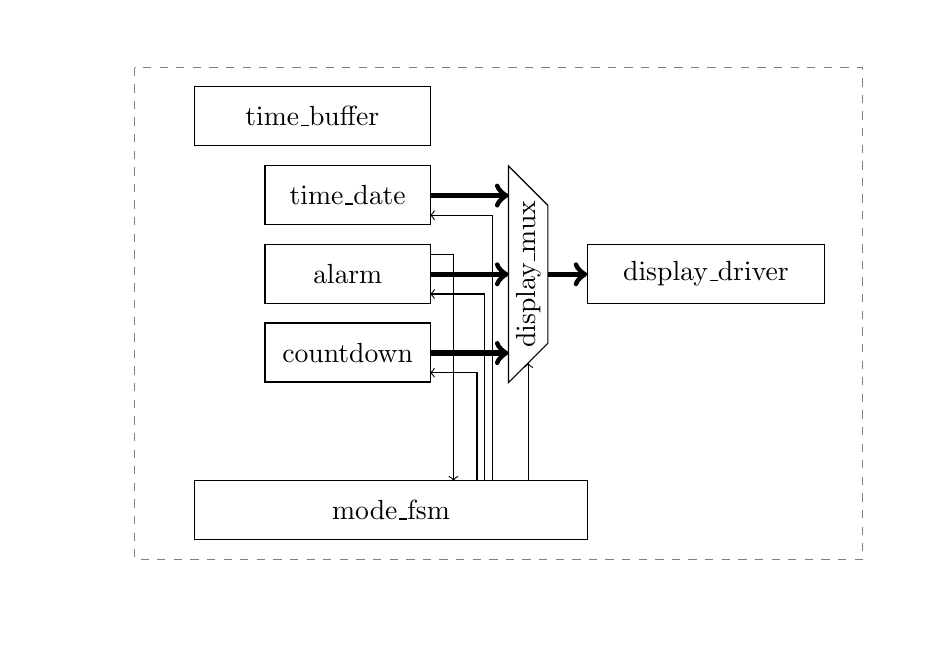
\begin{tikzpicture}
			\draw[white] (-2.1,.5) rectangle (9, -7);

		  % individual modules
		  \node[rectangle,draw=black,minimum height=.75cm,minimum width=3cm,above right] at (0,-1) {time\_buffer};
		  \node[rectangle,draw=black,minimum height=.75cm,minimum width=2.1cm,above right] at (.9,-2) {time\_date};
		  \node[rectangle,draw=black,minimum height=.75cm,minimum width=2.1cm,above right] at (.9,-3) {alarm};
		  \node[rectangle,draw=black,minimum height=.75cm,minimum width=2.1cm,above right] at (.9,-4) {countdown};
		  \node[rectangle,draw=black,minimum height=.75cm,minimum width=3cm,above right] at (5,-3) {display\_driver};
		  \node[rectangle,draw=black,minimum height=.75cm,minimum width=5cm,above right] at (0,-6) {mode\_fsm};

		  % display data signals
			\draw[line width=2pt,->] (3,-1.625) -> (4, -1.625);
			\draw[line width=2pt,->] (3,-2.625) -> (4, -2.625);
			\draw[line width=2pt,->] (3,-3.625) -> (4, -3.625);
			\draw[line width=2pt,->] (4.5,-2.625) -> (5, -2.625);

			% status signals modules -> fsm	
  		% only needed for alarm since we dropped the modified signal
			% \draw[->] (3,-1.375) -- (3.4,-1.375) -> (3.4,-5.25);
			\draw[->] (3,-2.375) -- (3.3,-2.375) -> (3.3,-5.25);
			% \draw[->] (3,-3.375) -- (3.2,-3.375) -> (3.2,-5.25);

			% control signals fsm -> modules
			\draw[->] (3.8,-5.25) -- (3.8,-1.875) -> (3,-1.875);
			\draw[->] (3.7,-5.25) -- (3.7,-2.875) -> (3,-2.875);
			\draw[->] (3.6,-5.25) -- (3.6,-3.875) -> (3,-3.875);

			% mux ctl
			\draw[->] (4.25,-5.25) -> (4.25,-3.75);


		  % mux
		  \draw (4,-1.25) -- (4.5, -1.75) -- (4.5,-3.5) -- (4,-4) -- cycle;
		  \node[rotate=90] at (4.25,-2.625) {display\_mux};

		  % top level module
		  \draw[dashed,gray] (-.75,0) rectangle (8.5, -6.25);
	  \end{tikzpicture}
  \end{frame}

  \begin{frame}{uhrenbaustein - supply input signals}
	  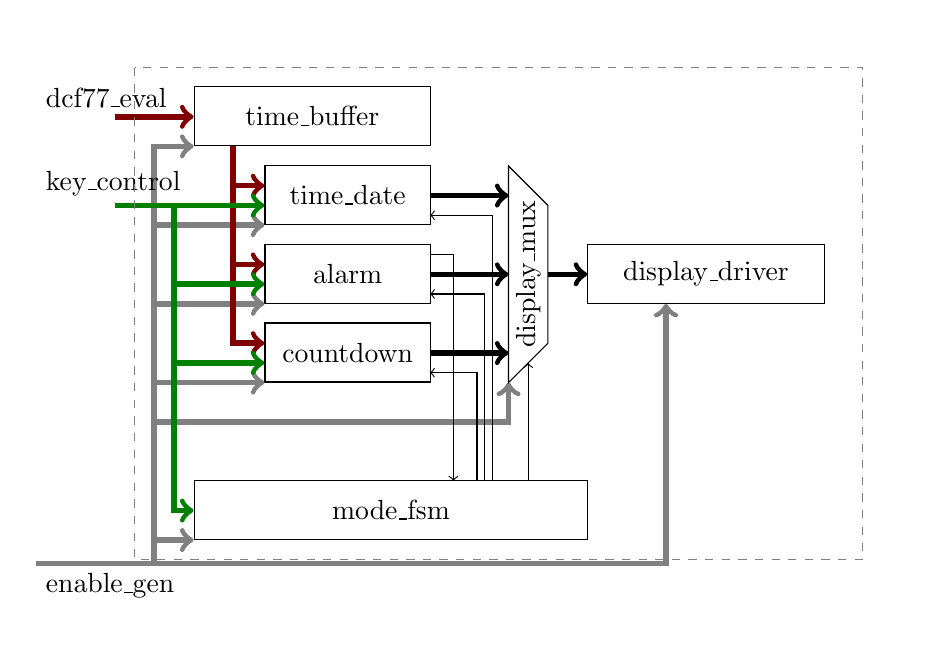
\begin{tikzpicture}
			\draw[white] (-2.1,.5) rectangle (9, -7);

		  % individual modules
		  \node[rectangle,draw=black,minimum height=.75cm,minimum width=3cm,above right] at (0,-1) {time\_buffer};
		  \node[rectangle,draw=black,minimum height=.75cm,minimum width=2.1cm,above right] at (.9,-2) {time\_date};
		  \node[rectangle,draw=black,minimum height=.75cm,minimum width=2.1cm,above right] at (.9,-3) {alarm};
		  \node[rectangle,draw=black,minimum height=.75cm,minimum width=2.1cm,above right] at (.9,-4) {countdown};
		  \node[rectangle,draw=black,minimum height=.75cm,minimum width=3cm,above right] at (5,-3) {display\_driver};
		  \node[rectangle,draw=black,minimum height=.75cm,minimum width=5cm,above right] at (0,-6) {mode\_fsm};

		  % clk/reset signals (enable_gen)
			\draw[white!50!black,line width=2pt,->] (-2,-6.3) -- (6,-6.3) ->  (6,-3);
			\draw[white!50!black,line width=2pt,->] (-.5,-6.3) -- (-.5,-1) -> (0,-1);
			\draw[white!50!black,line width=2pt,->] (-.5,-2) -> (.9,-2);
			\draw[white!50!black,line width=2pt,->] (-.5,-3) -> (.9,-3);
			\draw[white!50!black,line width=2pt,->] (-.5,-4) -> (.9,-4);
			\draw[white!50!black,line width=2pt,->] (-.5,-6) -> (0,-6);
			\draw[white!50!black,line width=2pt,->] (-.5,-4.5) -- (4,-4.5) -> (4,-4);
			\node[rectangle,below right] at (-2,-6.3) {enable\_gen};

		  % time signals
			\draw[red!50!black,line width=2pt,->] (-1,-.625) -- (0,-.625);
			\draw[red!50!black,line width=2pt,->] (.5,-1) -- (.5,-1.5) -> (.9,-1.5);
			\draw[red!50!black,line width=2pt,->] (.5,-1) -- (.5,-2.5) -> (.9,-2.5);
			\draw[red!50!black,line width=2pt,->] (.5,-1) -- (.5,-3.5) -> (.9,-3.5);
			\node[rectangle,above right] at (-2,-.625) {dcf77\_eval};

		  % key status signals
			\draw[green!50!black,line width=2pt,->] (-1,-1.75) -- (-.25,-1.75) -- (-.25,-1.75) -> (.9,-1.75);
			\draw[green!50!black,line width=2pt,->] (-1,-1.75) -- (-.25,-1.75) -- (-.25,-2.75) -> (.9,-2.75);
			\draw[green!50!black,line width=2pt,->] (-1,-1.75) -- (-.25,-1.75) -- (-.25,-3.75) -> (.9,-3.75);
			\draw[green!50!black,line width=2pt,->] (-1,-1.75) -- (-.25,-1.75) -- (-.25,-5.625) -> (0,-5.625);
			\node[rectangle,above right] at (-2,-1.75) {key\_control};

		  % display data signals
			\draw[line width=2pt,->] (3,-1.625) -> (4, -1.625);
			\draw[line width=2pt,->] (3,-2.625) -> (4, -2.625);
			\draw[line width=2pt,->] (3,-3.625) -> (4, -3.625);
			\draw[line width=2pt,->] (4.5,-2.625) -> (5, -2.625);
			% only needed for alarm since we dropped the modified signal
			% \draw[->] (3,-1.375) -- (3.4,-1.375) -> (3.4,-5.25);
			\draw[->] (3,-2.375) -- (3.3,-2.375) -> (3.3,-5.25);
			% \draw[->] (3,-3.375) -- (3.2,-3.375) -> (3.2,-5.25);

			% control signals fsm -> modules
			\draw[->] (3.8,-5.25) -- (3.8,-1.875) -> (3,-1.875);
			\draw[->] (3.7,-5.25) -- (3.7,-2.875) -> (3,-2.875);
			\draw[->] (3.6,-5.25) -- (3.6,-3.875) -> (3,-3.875);

			% mux ctl
			\draw[->] (4.25,-5.25) -> (4.25,-3.75);


		  % mux
		  \draw (4,-1.25) -- (4.5, -1.75) -- (4.5,-3.5) -- (4,-4) -- cycle;
		  \node[rotate=90] at (4.25,-2.625) {display\_mux};

		  % top level module
		  \draw[dashed,gray] (-.75,0) rectangle (8.5, -6.25);
	
    \end{tikzpicture}
  \end{frame}
 
  \begin{frame}{uhrenbaustein - supply output signals}
	  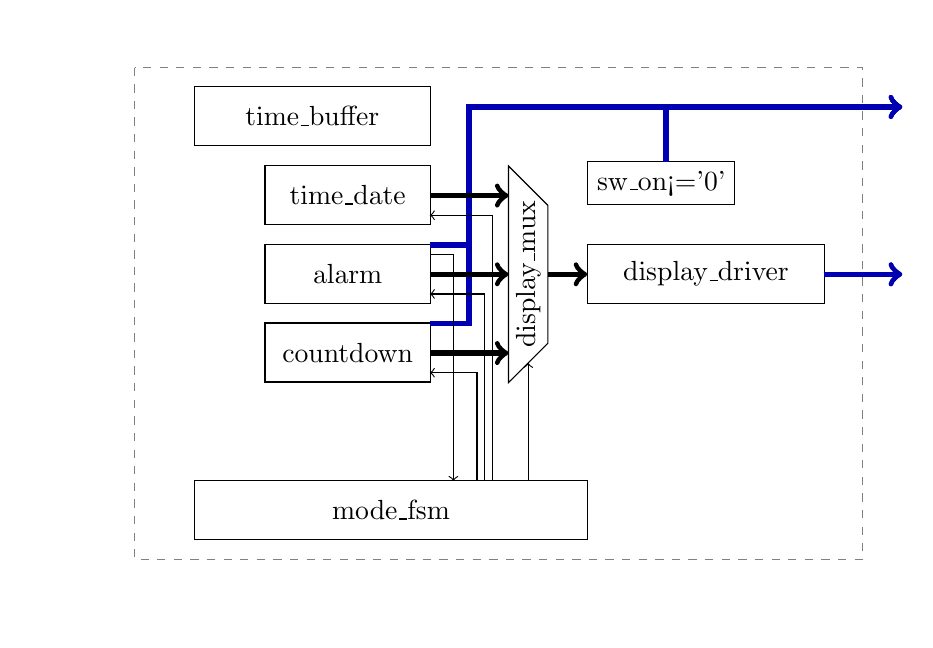
\begin{tikzpicture}
			\draw[white] (-2.1,.5) rectangle (9, -7);
	    % individual modules
	  	\node[rectangle,draw=black,minimum height=.75cm,minimum width=3cm,above right] at (0,-1) {time\_buffer};
		  \node[rectangle,draw=black,minimum height=.75cm,minimum width=2.1cm,above right] at (.9,-2) {time\_date};
		  \node[rectangle,draw=black,minimum height=.75cm,minimum width=2.1cm,above right] at (.9,-3) {alarm};
		  \node[rectangle,draw=black,minimum height=.75cm,minimum width=2.1cm,above right] at (.9,-4) {countdown};
		  \node[rectangle,draw=black,minimum height=.75cm,minimum width=3cm,above right] at (5,-3) {display\_driver};
		  \node[rectangle,draw=black,minimum height=.75cm,minimum width=5cm,above right] at (0,-6) {mode\_fsm};

	
      % outputs
		  \draw[blue!70!black,line width=2pt,->] (3,-2.25) -- (3.5,-2.25) -- (3.5,-.5) -> (9,-.5);
  	  \draw[blue!70!black,line width=2pt,->] (3,-3.25) -- (3.5,-3.25) -- (3.5,-.5) -> (9,-.5);
  	  \node[rectangle,draw=black,above right] at (5,-1.75) {sw\_on<='0'};
	    \draw[blue!70!black,line width=2pt,->] (6,-1.2) -- (6,-.5) -> (9,-.5);

		  % display control lines
	    \draw[blue!70!black,line width=2pt,->] (8,-2.625) -> (9,-2.625);

		  % display data signals
			\draw[line width=2pt,->] (3,-1.625) -> (4, -1.625);
			\draw[line width=2pt,->] (3,-2.625) -> (4, -2.625);
			\draw[line width=2pt,->] (3,-3.625) -> (4, -3.625);
			\draw[line width=2pt,->] (4.5,-2.625) -> (5, -2.625);
			% only needed for alarm since we dropped the modified signal
			% \draw[->] (3,-1.375) -- (3.4,-1.375) -> (3.4,-5.25);
			\draw[->] (3,-2.375) -- (3.3,-2.375) -> (3.3,-5.25);
			% \draw[->] (3,-3.375) -- (3.2,-3.375) -> (3.2,-5.25);


			% control signals fsm -> modules
			\draw[->] (3.8,-5.25) -- (3.8,-1.875) -> (3,-1.875);
			\draw[->] (3.7,-5.25) -- (3.7,-2.875) -> (3,-2.875);
			\draw[->] (3.6,-5.25) -- (3.6,-3.875) -> (3,-3.875);

			% mux ctl
			\draw[->] (4.25,-5.25) -> (4.25,-3.75);

			% display control lines
			\draw[blue!70!black,line width=2pt,->] (8,-2.625) -> (9,-2.625);

		  % mux
		  \draw (4,-1.25) -- (4.5, -1.75) -- (4.5,-3.5) -- (4,-4) -- cycle;
		  \node[rotate=90] at (4.25,-2.625) {display\_mux};

		  % top level module
		  \draw[dashed,gray] (-.75,0) rectangle (8.5, -6.25);
	
	\end{tikzpicture}
 \end{frame}
\section{mode\_alarm}
  \begin{frame}{mode\_alarm overview}
    \begin{tikzpicture}
      % main modules
		  \node[rectangle,draw=black,minimum height=1.5cm,minimum width=2.75cm,above right] at (0,2) {Alarm active};
	    \node[rectangle,draw=black,minimum height=1.5cm,minimum width=2.75cm,above right] at (0,-2) {Alarm time};
	    \node[rectangle,draw=black,minimum height=1.5cm,minimum width=2.75cm,above right] at (7,0) {AlarmOn FSM};
		  % compare
		  \draw (4,-.5) -- (4.5, -1) -- (4,-1.5) -- cycle;
      % OR
	    \node[rectangle,draw=black,minimum height=1cm,minimum width=1cm,above right] at (5.5,0.25) {OR};

%    \node[or gate US, draw,logic gate inputs=inini] (A) {;
%    \foreach \a in {1,\dots,5}
%        \draw (A.input \a -| -1,0) -- (A.input \a);
%        \draw (A.output) -- ([xshift=0.5cm]A.output);\\
%};

      % switch alarm active
		  \draw[->] (2.75,2.75)  -- (5,2.75)    -- (5,1)     -> (5.5,1);
		  \draw[->] (2.75,-1.25) -- (3.5,-1.25) -- (3.5, -1.25) -> (4,-1.25);
      \draw[->] (-1, 0)      -- (3.5,0)     -- (3.5, -0.75) -> (4,-0.75);
      \draw[->] (4.5, -1)    -- (5,-1)    -- (5, 0.5) -> (5.5,0.5);





    \end{tikzpicture}
  \end{frame}

  \begin{frame}{mode\_alarm FSM:alarm on}
		\begin{tikzpicture}[every state/.style={text width=1.3cm,align=center,node distance=.5cm},font=\tiny,auto]
		  \node[right,text width=100cm,align=left] at (2,1.5) {All transitions occur on CLK$\uparrow$};
		  \node[state,                              minimum size=2.3cm](AlarmOnA) { ALARM ON   \\ al\_on = 1 \\ alarm\_on = 1 \\ snooze <= alarm\_time };
		  \node[state,right=of AlarmOnA,xshift=2cm, minimum size=2.3cm](Snooze)   { SNOOZE     \\ al\_on = 0 \\ alarm\_on = 0 \\ snooze <= current\_time + 5min };
		  \node[state,below=of Snooze,  yshift=-1cm,minimum size=2.3cm](AlarmOnB) { ALARM ON   \\ al\_on = 1 \\ alarm\_on = 1 \\ };
		  \node[state,below=of AlarmOnA,yshift=-1cm,minimum size=2.3cm](AlarmOff) { ALARM OFF  \\ al\_on = 0 \\ alarm\_on = 0 \\ };

		  \path[->] (AlarmOnA) ++(-3,0) edge (AlarmOnA)
		            (AlarmOnA)     edge             node {kc\_act\_imp}                 (Snooze)
		            (AlarmOnA)     edge[bend right] node {kc\_act\_long}                (AlarmOff)
              	(AlarmOnA)     edge[bend left]  node { >1min}                       (AlarmOff)
		            (AlarmOnB)     edge[bend left]  node {kc\_act\_imp}                 (Snooze)
		            (AlarmOnB)     edge[bend left]  node {kc\_act\_long}                (AlarmOff)
  	            (AlarmOnB)     edge[bend right] node {>1min}                        (AlarmOff)
                (Snooze)       edge[bend left]  node {snooze=current\_time}         (AlarmOnB);



	  \end{tikzpicture}
  \end{frame}
\end{document}

